\documentclass{article}

\usepackage[margin=.75in]{geometry}
\usepackage{amsmath}
\usepackage{amssymb}
\usepackage[shortlabels]{enumitem}
\usepackage{pgfplots}
\usepackage{circuitikz}
\usepackage{float}

\author{Damien Prieur}
\title{Final Part 1\\ ECES 511}
\date{}

\begin{document}

\maketitle

\section*{Problem 1}
Determine the convolution of the two signals $p(t)$ and $g(t)$ below.
You can either plot or write down the equation for your answer.
Show all your work and clearly indicate your answer.
\begin{figure}[h!]
\centering
\begin{tikzpicture}[>=stealth]
    \begin{axis}[
        xmin=-.5,xmax=4.5,
        ymin=-.5,ymax=2,
        axis x line=middle,
        axis y line=middle,
        axis line style=->,
        xlabel={$t$},
        ylabel={$p(t)$},
        width=0.45\textwidth,
        height=0.25\textwidth,
        ]
        \addplot[no marks,black,-] expression[domain=0:1,samples=20]{1};
        \addplot[no marks,black,-]coordinates {(1,0)(1,1)};
    \end{axis}
\end{tikzpicture}
\centering
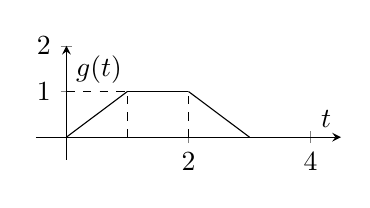
\begin{tikzpicture}[>=stealth]
    \begin{axis}[
        xmin=-.5,xmax=4.5,
        ymin=-.5,ymax=2,
        axis x line=middle,
        axis y line=middle,
        axis line style=->,
        xlabel={$t$},
        ylabel={$g(t)$},
        width=0.45\textwidth,
        height=0.25\textwidth,
        ]
        \addplot[no marks,black, dashed]coordinates {(0,1)(1,1)};
        \addplot[no marks,black,-]coordinates {(0,0)(1,1)};
        \addplot[no marks,black, dashed]coordinates {(1,0)(1,1)};
        \addplot[no marks,black,-]coordinates {(1,1)(2,1)};
        \addplot[no marks,black, dashed]coordinates {(2,0)(2,1)};
        \addplot[no marks,black,-]coordinates {(2,1)(3,0)};
    \end{axis}
\end{tikzpicture}
\end{figure}
We have
$$
y(t) = \int_{0}^{t} g(\tau)p(t-\tau) d\tau
$$
$$
g(t)
=
\begin{cases}
    t       & 0 \leq t \leq 1 \\
    1       & 1 \le  t \leq 2 \\
    -(t-3)  & 2 \le  t \leq 3 \\
    0   & otherwise
\end{cases}
\quad
p(t)
=
\begin{cases}
    1   & 0 \leq t \leq 1 \\
    0   & otherwise
\end{cases}
$$
$$
y(t) = \int_{0}^{t} g(t-\tau)u(\tau) d\tau
=
\begin{cases}
    \int_{0}^{t} \tau d\tau & 0 \leq t \leq 1 \\
    \int_{t-1}^{1} \tau d\tau + \int_{1}^{t} p(t-\tau) d\tau  & 1 \leq t \leq 2 \\
    \int_{t-1}^{2} p(t-\tau) d\tau + \int_{2}^{t} -(\tau -3) p(t-\tau)d\tau  & 2 \leq t \leq 3 \\
    \int_{t-1}^{3} -(\tau-3)p(t-\tau) d\tau & 3 \leq t \leq 4 \\
    0   & otherwise
\end{cases}
$$
$$y(t) =
\begin{cases}
    \frac{ t^2}{2}          & 0 \leq t \leq 1 \\
    \frac{-t^2}{2} + 2t - 1 & 1 \leq t \leq 2 \\
    \frac{-t^2}{2} + 2t - 1 & 2 \le  t \leq 3 \\
    \frac{ t^2}{2} - 4t + 8 & 3 \le  t \leq 4 \\
    0   & otherwise
\end{cases}
$$
\begin{figure}[h!]
\centering
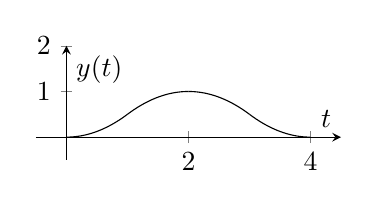
\begin{tikzpicture}[>=stealth]
    \begin{axis}[
        xmin=-.5,xmax=4.5,
        ymin=-.5,ymax=2,
        axis x line=middle,
        axis y line=middle,
        axis line style=->,
        xlabel={$t$},
        ylabel={$y(t)$},
        width=.45\textwidth,
        height=0.25\textwidth,
        ]
        \addplot[no marks,black,-] expression[domain=0:1,samples=30]{x*x/2};
        \addplot[no marks,black,-] expression[domain=1:2,samples=30]{-x*x/2 + 2*x -1};
        \addplot[no marks,black,-] expression[domain=2:3,samples=30]{-x*x/2 + 2*x -1};
        \addplot[no marks,black,-] expression[domain=3:4,samples=30]{x*x/2 - 4*x +8};
    \end{axis}
\end{tikzpicture}
\end{figure}


\newpage
\section*{Problem 2}
Let $v_1=\begin{bmatrix} 1 \\ 3 \\ 5 \end{bmatrix}$,$v_2=\begin{bmatrix} 2 \\ 5 \\ 9 \end{bmatrix}$,$v_2=\begin{bmatrix} -3 \\ 9 \\ 3 \end{bmatrix}$,
\begin{enumerate}[1)]
\item Determine if $\{v_1,v_2,v_3\}$ is linearly independent?
\newline
We can check for independence by performing Gaussian elimination of the matrix comprised of $[v_1 \quad v_2 \quad v_3]$
$$
A =
\begin{bmatrix}
1 & 2 & -3 \\
3 & 5 & 9  \\
5 & 9 & 3
\end{bmatrix}
$$
$$
\begin{bmatrix}
1 & 2 & -3 \\
3 & 5 & 9  \\
5 & 9 & 3
\end{bmatrix}
\implies
\begin{bmatrix}
1 & 2  & -3  \\
0 & -1 & -18 \\
0 & -1 & -12
\end{bmatrix}
\implies
\begin{bmatrix}
1 & 2  & -3  \\
0 & -1 & -18 \\
0 & 0  & -6
\end{bmatrix}
$$
Since we have reduced this to an upper triangular matrix each column is linearly independent from each other.
This implies that the rank of the matrix is $3$.
\item If it is linearly independent find $a$, $b$, $c$ where $av_1 + bv_2 + cv_3 = 0$.
If not, find the relations among $v_1,v_2,v_3$.
\newline
Since all the columns are linearly independent and the rank matches the dimensions of the matrix the null space of $A$ only contains the zero vector.
$$
\begin{bmatrix}a\\b\\c\end{bmatrix}
=
\begin{bmatrix}0\\0\\0\end{bmatrix}
$$
\end{enumerate}

\newpage
\section*{Problem 3}
Given 5 equations:
\begin{align*}
 2a + b &= 20 \\
 6a + b &= 18 \\
20a + b &= 10 \\
30a + b &=  6 \\
40a + b &=  2 \\
\end{align*}
\begin{enumerate}[a)]
\item Find the closest solution $\{a,b\}$ to the five equations.
{\color{blue} Use MATLAB to confirm how "close" it is.}
\newline
If we rewrite the equations into matrix form $Ax=b$
$$
A=
\begin{bmatrix}
2 & 1 \\
6 & 1 \\
20 & 1 \\
30 & 1 \\
40 & 1 \\
\end{bmatrix}
\qquad
x =
\begin{bmatrix} a \\ b \end{bmatrix}
\qquad
b =
\begin{bmatrix}
20 \\
18 \\
10 \\
6  \\
2  \\
\end{bmatrix}
$$
We can solve this equation by performing the pseudoinverse and modifying our original equation with $A^TAx=A^Tb \implies x = (A^TA)^{-1}A^Tb$
\newline
First we compute $A^TA$
$$
A^TA
=
\begin{bmatrix}
2 & 6 & 20 & 30 & 40 \\
1 & 1 & 1 & 1 & 1 \\
\end{bmatrix}
\begin{bmatrix}
2  & 1 \\
6  & 1 \\
20 & 1 \\
30 & 1 \\
40 & 1 \\
\end{bmatrix}
=
\begin{bmatrix}
2940  & 98 \\
98  & 5 \\
\end{bmatrix}
$$
Now we can find the inverse of $A^TA$
$$(A^TA)^{-1}
=
\frac{1}{det(A^TA)}
adj(A^TA)
=
\frac{1}{5096}
\begin{bmatrix}
5 & -98 \\
-98 & 2940 \\
\end{bmatrix}
$$
$$
x = (A^TA)^{-1}A^Tb
=
\frac{1}{5096}
\begin{bmatrix}
5 & -98 \\
-98 & 2940 \\
\end{bmatrix}
\begin{bmatrix}
2 & 6 & 20 & 30 & 40 \\
1 & 1 & 1 & 1 & 1 \\
\end{bmatrix}
\begin{bmatrix}
20 \\
18 \\
10 \\
6  \\
2  \\
\end{bmatrix}
=
\frac{1}{5096}
\begin{bmatrix}
5 & -98 \\
-98 & 2940 \\
\end{bmatrix}
\begin{bmatrix}
608 \\
56
\end{bmatrix}
=
\frac{1}{5096}
\begin{bmatrix}
-2448 \\
105056
\end{bmatrix}
$$
$$
\begin{bmatrix}
a\\
b
\end{bmatrix}
=
\begin{bmatrix}
-0.480377 \\
20.615385
\end{bmatrix}
$$
My error using squared error $(Ax-b)^T(Ax-b)$ was $1.6075$ while matlab's solution using $pinv(A)*x$ was also $1.6075$ and also came to the same numerical solution.


\item Is there any geometric meaning for $\{a,b\}$?
\newline
Each equation can be thought of as a line in the plane and our solution is the point that minimizes the squared error for all equations.
\end{enumerate}

\newpage
\section*{Problem 4}
Using the transfer function $\frac{Y(s)}{R(s)} = \frac{6}{(s+2)(s+3)}$.
\newline
Note this transfer function has no zero/pole cancellation and is a minimal polynomial.
\begin{enumerate}[1)]
\item Convert from Transfer function to Differential equation then to the State equations.
\newline
Separating the transfer function we get
$$ Y(s)(s^2+5s+6) = 6R(s) $$
Taking the inverse Laplace transform on each side we get
$$\ddot{y} + 5 \dot{y} + 6y = 6r $$
Let $x_1 = y \quad x_2 = \dot{y}$
Now converting the Differential equation to state space form we get.
$$
\begin{bmatrix}
\dot{x}_1 \\
\dot{x}_2
\end{bmatrix}
=
\begin{bmatrix}
x_2 \\
6 r -5x_2 -6x_1
\end{bmatrix}
\qquad
y = x_1
$$
In Matrix form we get
$$
\begin{bmatrix}
\dot{x}_1 \\
\dot{x}_2
\end{bmatrix}
=
\begin{bmatrix}
0 & 1 \\
-6 & -5 
\end{bmatrix}
x +
\begin{bmatrix}
0 \\
6
\end{bmatrix}
r(t)
$$
$$
y = \begin{bmatrix} 1 & 0 \end{bmatrix} x
$$
\item Confirm by converting directly from the Transfer function to the State equation.
{\color{blue} Use MATLAB to confirm.}
\newline
Writing the Transfer Function in matrix form with $Q_1(s) = Y(S) \quad Q_2(s) = sY(S)$
$$
s
\begin{bmatrix}
Q_1(s) \\
Q_2(s)
\end{bmatrix}
=
\begin{bmatrix}
0 & 1 \\
-6 & -5
\end{bmatrix}
Q(s)
+
\begin{bmatrix}
0 \\
6
\end{bmatrix}
R(s)
$$
$$ Y(s) = \begin{bmatrix} 1 & 0 \end{bmatrix} Q(s) $$
Now if we take the inverse laplace transform of this system we get
$$
\begin{bmatrix}
\dot{y} \\
\ddot{y}
\end{bmatrix}
=
\begin{bmatrix}
0 & 1 \\
-6 & -5
\end{bmatrix}
y
+
\begin{bmatrix}
0 \\
6
\end{bmatrix}
r(t)
$$
$$ y = \begin{bmatrix} 1 & 0 \end{bmatrix} y(t) $$
If we use the same substitution as in part 1 we get the same system of equations out.
\item Calculate the impulse response of the system.
\newline
Since we have the transfer function $H(s)$ if we take it's inverse Laplace transform we get the impulse response $h(t)$
$$H(s) = \frac{6}{s^2 + 5s + 6}$$
Breaking this up into two fractions we get
$$ H(s) = 6(\frac{1}{2+s} - \frac{1}{3+s}) $$
Taking the inverse Laplace transform gives us
$$ h(t) = 6(e^{-2 t} - e^{-3 t}) $$
\end{enumerate}

\newpage
\section*{Problem 5}
Use the Cayley Hamilton Theorem to find $A^{-1}$ where $A = \begin{bmatrix} 0 & 1 \\ -2 & 3 \end{bmatrix}$.
Validate your answer with $AA^{-1}$.
\newline
Let $f(\lambda)=\lambda^{-1}$
Finding the eigenvalues of $A$
$$det(A - \lambda I) =
\begin{vmatrix}
-\lambda & 1 \\
-2 & 3 - \lambda
\end{vmatrix}
=
\lambda^2 - 3\lambda + 2
=
(\lambda - 1)(\lambda - 2)
$$
$$ \lambda_1 = 1 \qquad \lambda_2 = 2 $$
Let $h(\lambda) = \beta_0 + \beta_1 \lambda$
Since each eigenvalue have multiplicity 1 we get one equation from each.
$$ h(\lambda_1) = f(\lambda_1) \implies \beta_0 + \beta_1(1) = (1)^{-1} = 1 $$
$$ h(\lambda_2) = f(\lambda_2) \implies \beta_0 + \beta_1(2) = (2)^{-1} = \frac{1}{2} $$
Solving for $\beta_0$ with the first equation and substituting into the second equation we get a solution.
$$\beta_0 = 1 - \beta_1$$  
$$ 1 -\beta_1 + 2\beta_1 = \frac{1}{2} \implies \beta_1 = -\frac{1}{2}$$
$$\implies \beta_0 = \frac{3}{2} $$
Plugging in the values for $\beta$ we get
$$ h(\lambda) = \frac{3}{2} - \frac{1}{2} \lambda $$
And finally finding $ f(A) = h(A) = A^{-1} $
$$ A^{-1} =
\frac{1}{2}
(
\begin{bmatrix}
3 & 0 \\
0 & 3
\end{bmatrix}
-
\begin{bmatrix}
0 & 1 \\
-2 & 3
\end{bmatrix}
)
=
\frac{1}{2}
\begin{bmatrix}
3 & -1 \\
2 & 0
\end{bmatrix}
$$
Confirming the solution by verifying $AA^{-1} = I$
$$
\frac{1}{2}
\begin{bmatrix}
0 & 1 \\
-2 & 3
\end{bmatrix}
\begin{bmatrix}
3 & -1 \\
2 & 0
\end{bmatrix}
=
\begin{bmatrix}
1 & 0 \\
0 & 1
\end{bmatrix}
$$

\newpage
\section*{Problem 6}
Given the following system with initial conditions:
\begin{align*}
\frac{dx}{dt} &= \begin{bmatrix} -2 & 0 \\ 0 & -4 \end{bmatrix} x(t) + \begin{bmatrix} 4 \\ -1 \end{bmatrix} r(t) \\
y(t) &= \begin{bmatrix} 1 & 3 \end{bmatrix} x(t) \\
x(0) &= \begin{bmatrix} 4 \\ 5 \end{bmatrix} \\
\end{align*}
\begin{enumerate}[a)]
\item Find the state transition matrix $\varphi (t) = e^{At}$.
{\color{blue} Use MATLAB to confirm}
\newline
Since our original matrix is already in it's Jordan diagonal form computing $e^{At}$ is trivial by taking each diagonal term to $e^{at}$
$$\varphi (t) = e^{At} =
\begin{bmatrix}
e^{-2t} & 0 \\
0 & e^{-4t}
\end{bmatrix}
$$
\item Find the transfer function $\frac{Y(s)}{R(s)}$ (factor all polynomials).
\newline
The transfer function can be found with this relationship $\frac{Y(s)}{R(s)} = C\Phi(s)B  + D $ where  $\Phi(s) = (sI - A)^{-1}$
$$\Phi (s) =
(\begin{bmatrix}
s & 0 \\
0 & s
\end{bmatrix}
-
\begin{bmatrix}
-2 & 0 \\
0 & -4
\end{bmatrix}
)^{-1}
=
(
\begin{bmatrix}
s+2 & 0 \\
0 & s+4
\end{bmatrix}
)^{-1}
=
\frac{1}{(s+4)(s+2)}
\begin{bmatrix}
s+4 & 0 \\
0 & s+2
\end{bmatrix}
$$
Now computing the transfer function we get
$$
\frac{Y(s)}{R(s)}
=
\frac{1}{(s+4)(s+2)}
\begin{bmatrix}
1 & 3
\end{bmatrix}
\begin{bmatrix}
s+4 & 0 \\
0 & s+2
\end{bmatrix}
\begin{bmatrix}
4 \\
-1
\end{bmatrix}
=
\frac{1}{(s+4)(s+2)}
\begin{bmatrix}
1 & 3
\end{bmatrix}
\begin{bmatrix}
4s+16\\
-s-2
\end{bmatrix}
$$
$$
\frac{Y(s)}{R(s)}
=
\frac{4s+16 -3s -6}{(s+4)(s+2)}
=
\frac{s+10}{(s+4)(s+2)}
$$

\item Find the total solution for the state vector $x(t)$ if the input $r(t) = 2 u(t)$ where $u(t) = unit step function$.
{\color{blue} Use MATLAB to confirm}
\newline
\hspace*{10mm} Clearly identify the \textbf{zero input part} of the solution
\newline
\hspace*{10mm} Clearly identify the \textbf{zero state part} of the solution
\newline
\hspace*{10mm} Then combine into a final result
\newline
Show the results in both the time domain and Laplace domain.
\textbf{Hint:} It is easier to solve if you work in the Laplace domain then convert to the time domain.
\newline
The close form solution is given by $Y(s) = C \Phi(s)(X(0) + BR(s))$
$$R(s) = \mathcal{L}\{2u(t)\} = \frac{2}{s} \qquad \Phi(s) =
\frac{1}{(s+4)(s+2)}
\begin{bmatrix}
s+4 & 0 \\
0 & s+2
\end{bmatrix}
$$
$$Y(s) = C\Phi(s)X(0) +C\Phi(s)BR(s)$$
The first term is the zero input term and the second term is the zero state term.
Computing each individually we have
$$Y_{zi}(s)  = C\Phi(s)X(0) = \frac{4}{s+2} + \frac{15}{s+4} $$
$$Y_{zs}(s)  = C\Phi(s)BR(s) = \frac{2}{s}(\frac{4}{s+2} - \frac{3}{s+4})  =  \frac{5}{2 s}-\frac{4}{s+2}+\frac{3}{2 (s+4)}$$
To find $y(t)$ we take the inverse Laplace transform of $Y(s)$.
$$
y_{zi}(t)
=
\mathcal{L}^{-1}\{Y_{zi}(s)\}
=
\mathcal{L}^{-1}\{\frac{4}{s+2} + \frac{15}{s+4}\}
=
15 e^{-4t} + 4 e^{-2t}
$$
$$
y_{zi}(t)
=
15 e^{-4t} + 4 e^{-2t}
$$
$$
y_{zs}(t)
=
\mathcal{L}^{-1}\{Y_{zs}(s)\}
=
\mathcal{L}^{-1}\{\frac{5}{4s} - \frac{4}{2+s} + \frac{3}{2(s+4)}\}
=
\frac{5}{2} + \frac{3}{2}e^{-4t} - 4 e^{-2t}
$$
$$
y_{zs}(t)
=
\frac{5}{2} + \frac{3}{2}e^{-4t} - 4 e^{-2t}
$$
Combining the zero state and zero input solutions we get the solution to be
$$ y(t) = \frac{5}{2} + \frac{33}{2}e^{-4t} $$
If we compare the results of lsim to our solution we see they match 
\begin{figure}[h!]
\includegraphics[scale=.75]{{images/p6_lsim}.png}
\end{figure}
\end{enumerate}

\newpage
\section*{Problem 7}
Use the same system in Problem 6
\begin{enumerate}[a)]
\item Use MATLAB to plot the state variables in continuous time over the time range $t \in [0,10]$
\newline
\begin{figure}[h!]
\centering
\includegraphics[scale=.3]{{images/p7_lsim}.png}
\end{figure}
\item Calculate the $A_d, B_d, C_d, D_d$ for discrete system if sampled at $T = \frac{1}{2}$s.
\newline
From problem 6 part a we already have $e^{At}$ so
$$A_d = e^{AT} = \varphi(\frac{1}{2}) =
\begin{bmatrix}
e^{-1} & 0 \\
0 & e^{-2}
\end{bmatrix}
$$
$$
B_d = (\int_0^T e^{A\alpha}d\alpha)B =
\begin{bmatrix}
\frac{-1}{2}e^{-1} + \frac{1}{2} & 0 \\
0 & \frac{-1}{4}e^{-2} + \frac{1}{4} 
\end{bmatrix}
\begin{bmatrix}
4 \\
-1
\end{bmatrix}
=
\begin{bmatrix}
-2e^{-1} + 2 \\
\frac{1}{4}e^{-2} - \frac{1}{4}
\end{bmatrix}
$$
$$ C_d = C = \begin{bmatrix} 1 & 3 \end{bmatrix} $$
$$ D_d = D = 0 $$
\item Use MATLAB to plot the discrete response of the same state variable as (a) and compare the two plots.
\newline
We can see that at each evaluation of the discrete model it's extremely close to the continuous model and exactly the same for $x_1$.
\begin{figure}[h!]
\centering
\includegraphics[scale=.5]{{images/p8_lsim}.png}
\end{figure}

\end{enumerate}

\newpage
\section*{Problem 8}
Compute the singular value decomposition of $A = \begin{bmatrix} 2 & 0 & 0 \\ 0 & 2 & 1 \\ 0 & 1 & 2 \\ 0 & 0 & 0 \end{bmatrix}$.
{\color{blue} Use MATLAB to confirm.}
\newline
First we compute $A^TA$
$$A^TA =
\begin{bmatrix}
2 & 0 & 0 & 0 \\
0 & 2 & 1 & 0 \\
0 & 1 & 2 & 0 \\
\end{bmatrix}
\begin{bmatrix}
2 & 0 & 0 \\
0 & 2 & 1 \\
0 & 1 & 2 \\
0 & 0 & 0
\end{bmatrix}
=
\begin{bmatrix}
4 & 0 & 0 \\
0 & 5 & 4 \\
0 & 4 & 5
\end{bmatrix}
$$
Next we find the eigenvalues for $A^TA$
$$det(A^TA - \lambda I)
=
\begin{vmatrix}
4-\lambda & 0 & 0 \\
0 & 5-\lambda & 4 \\
0 & 4 & 5-\lambda
\end{vmatrix}
=
(4-\lambda)((5-\lambda)^2-16)
=-\lambda ^3+14 \lambda ^2-49 \lambda +36
=-(\lambda -9) (\lambda -4) (\lambda -1)
$$
$$ \lambda_1 = 9 \qquad \lambda_2 = 4 \qquad \lambda_3 = 1 $$
We get the singular values by taking the square root of the eigenvalues
$$ \sigma_1 = 3 \qquad \sigma_2 = 2 \qquad \sigma_3 = 1 $$
$$
\Sigma =
\begin{bmatrix}
3 & 0 & 0 \\
0 & 2 & 0 \\
0 & 0 & 1 \\
0 & 0 & 0
\end{bmatrix}
$$
Getting $V$ we find the eigenvectors of $A^TA$
$$
\lambda_1 = 9 \implies
\begin{bmatrix}
-5 & 0 & 0 \\
0 & -4 & 4 \\
0 & 4 & -4
\end{bmatrix}
x
=0
\implies q_1 =
\frac{1}{\sqrt{2}}
\begin{bmatrix}
0 \\
1 \\
1
\end{bmatrix}
$$
$$
\lambda_2 = 4 \implies
\begin{bmatrix}
0 & 0 & 0 \\
0 & 1 & 4 \\
0 & 4 & 1
\end{bmatrix}
x
=0
\implies q_2 =
\begin{bmatrix}
1 \\
0 \\
0
\end{bmatrix}
$$
$$
\lambda_3 = 1 \implies
\begin{bmatrix}
3 & 0 & 0 \\
0 & 4 & 4 \\
0 & 4 & 4
\end{bmatrix}
x
=0
\implies q_3 =
\frac{1}{\sqrt{2}}
\begin{bmatrix}
0 \\
1 \\
-1
\end{bmatrix}
$$
Combining these terms so the matrix is also unit magnitude we get
$$
V =
\frac{1}{\sqrt{2}}
\begin{bmatrix}
0 & \sqrt{2} & 0 \\
1 & 0 & 1 \\
1 & 0 & -1
\end{bmatrix}
$$
Finding each column of $U$ with the relationship $u_i = \sigma_i^{-1}Av_i$
$$u_1 =
\frac{1}{3}
\begin{bmatrix}
2 & 0 & 0 \\
0 & 2 & 1 \\
0 & 1 & 2 \\
0 & 0 & 0
\end{bmatrix}
\begin{bmatrix}
0 \\
1 \\
1
\end{bmatrix}
=
\begin{bmatrix}
0 \\
1 \\
1 \\
0
\end{bmatrix}
$$
$$u_2 =
\frac{1}{2}
\begin{bmatrix}
2 & 0 & 0 \\
0 & 2 & 1 \\
0 & 1 & 2 \\
0 & 0 & 0
\end{bmatrix}
\begin{bmatrix}
1 \\
0 \\
0
\end{bmatrix}
=
\begin{bmatrix}
1 \\
0 \\
0 \\
0
\end{bmatrix}
$$
$$u_3 =
\begin{bmatrix}
2 & 0 & 0 \\
0 & 2 & 1 \\
0 & 1 & 2 \\
0 & 0 & 0
\end{bmatrix}
\begin{bmatrix}
0 \\
1 \\
-1
\end{bmatrix}
=
\begin{bmatrix}
0 \\
1 \\
-1 \\
0
\end{bmatrix}
$$
The last column $u_4$ needs to be linearly independent from the other columns so taking the easiest solution we find
$$u_4 =
\begin{bmatrix}
0 \\
0 \\
0 \\
1 \\
\end{bmatrix}
$$
Combining the columns and making them all unit magnitude we get
$$ U =
\frac{1}{\sqrt{2}}
\begin{bmatrix}
0 & \sqrt{2} & 0 & 0 \\
1 & 0 & 1 & 0 \\
1 & 0 & -1 & 0 \\
0 & 0 & 0 & 1 \\
\end{bmatrix}
$$
So we have but the columns are correct up to the sign so we just need to test to determine the sign for each column to recreate $A$
$$
A = U\Sigma V^T =
\frac{1}{\sqrt{2}}
\begin{bmatrix}
0 & \sqrt{2} & 0 & 0\\
-1 & 0 & -1 & 0\\
-1 & 0 & 1 & 0\\
0 & 0 & 0 & \sqrt{2}\\
\end{bmatrix}
\begin{bmatrix}
3 & 0 & 0 \\
0 & 2 & 0 \\
0 & 0 & 1 \\
0 & 0 & 0
\end{bmatrix}
\frac{1}{\sqrt{2}}
\begin{bmatrix}
0 & -1 & -1 \\
\sqrt{2} & 0 & 0 \\
0 & -1 & 1
\end{bmatrix}
$$
Evaluating this we can confirm that this equals $A$
$$
\frac{1}{\sqrt{2}}
\begin{bmatrix}
0 & \sqrt{2} & 0 & 0\\
-1 & 0 & -1 & 0\\
-1 & 0 & 1 & 0\\
0 & 0 & 0 & \sqrt{2}\\
\end{bmatrix}
\begin{bmatrix}
3 & 0 & 0 \\
0 & 2 & 0 \\
0 & 0 & 1 \\
0 & 0 & 0
\end{bmatrix}
\frac{1}{\sqrt{2}}
\begin{bmatrix}
0 & -1 & -1 \\
\sqrt{2} & 0 & 0 \\
0 & -1 & 1
\end{bmatrix}
=
\begin{bmatrix}
2 & 0 & 0 \\
0 & 2 & 1 \\
0 & 1 & 2 \\
0 & 0 & 0
\end{bmatrix}
$$



\end{document}
